\documentclass{standalone}
\usepackage{tikz}
\usetikzlibrary{patterns, positioning}


\begin{document}
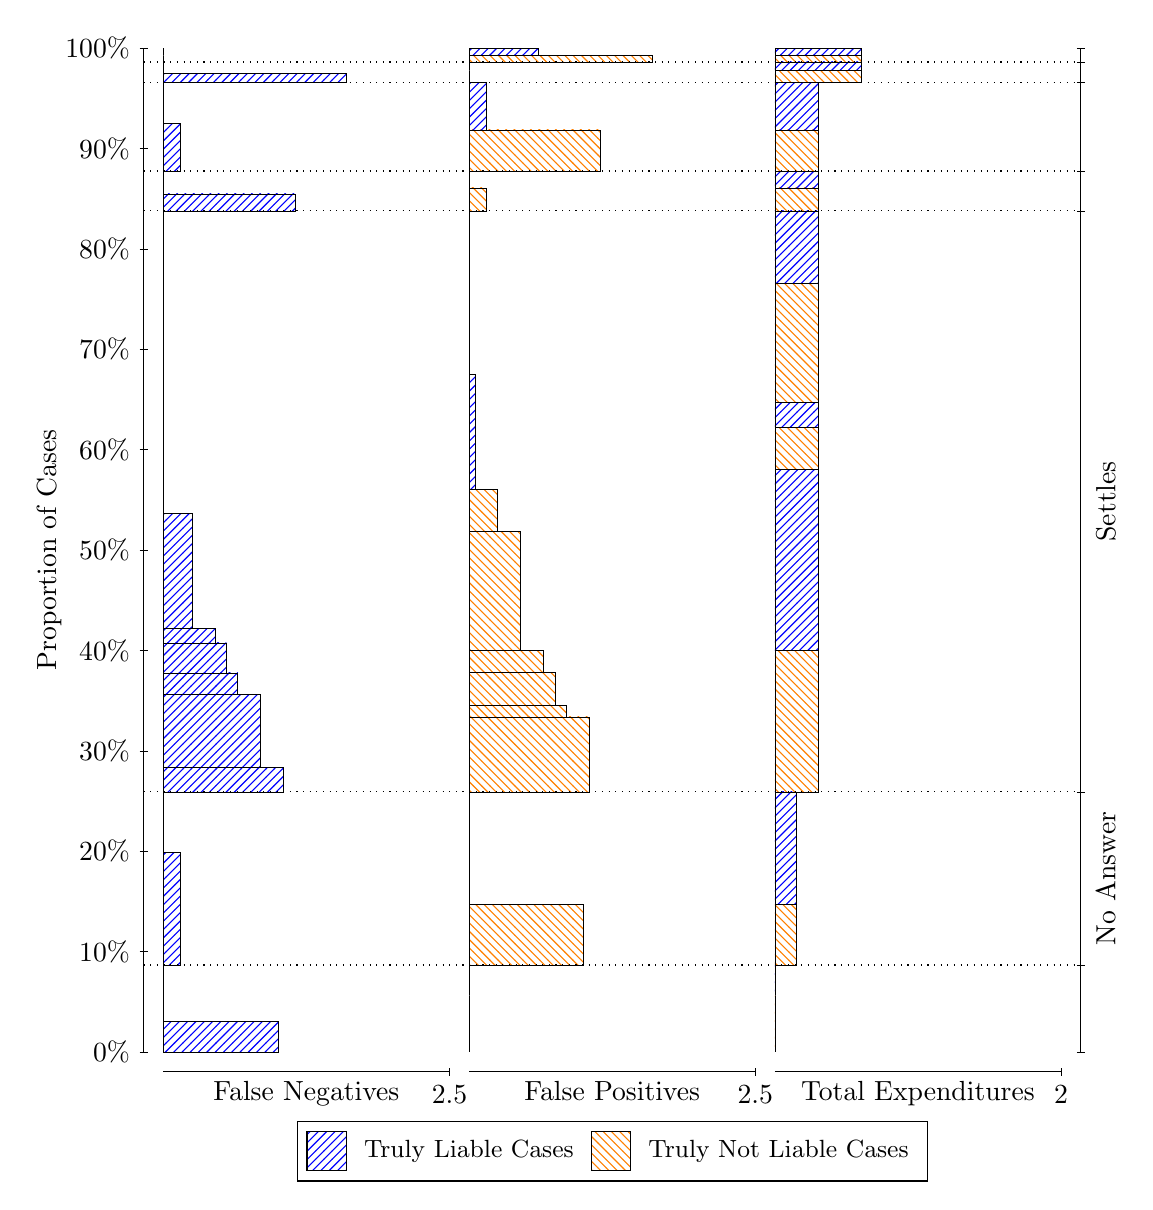
\begin{tikzpicture}
\draw[black, very thin] (1.5,1.75) -- (1.5,14.5);
\node[rotate=90, text=black, anchor=center] at (0.3, 8.125) {Proportion of Cases};
\draw[black, very thin] (1.45,1.75) -- (1.55,1.75);
\node[text=black, anchor=east] at (1.45, 1.75) {0\%};
\draw[black, very thin] (1.45,3.025) -- (1.55,3.025);
\node[text=black, anchor=east] at (1.45, 3.025) {10\%};
\draw[black, very thin] (1.45,4.3) -- (1.55,4.3);
\node[text=black, anchor=east] at (1.45, 4.3) {20\%};
\draw[black, very thin] (1.45,5.575) -- (1.55,5.575);
\node[text=black, anchor=east] at (1.45, 5.575) {30\%};
\draw[black, very thin] (1.45,6.85) -- (1.55,6.85);
\node[text=black, anchor=east] at (1.45, 6.85) {40\%};
\draw[black, very thin] (1.45,8.125) -- (1.55,8.125);
\node[text=black, anchor=east] at (1.45, 8.125) {50\%};
\draw[black, very thin] (1.45,9.4) -- (1.55,9.4);
\node[text=black, anchor=east] at (1.45, 9.4) {60\%};
\draw[black, very thin] (1.45,10.675) -- (1.55,10.675);
\node[text=black, anchor=east] at (1.45, 10.675) {70\%};
\draw[black, very thin] (1.45,11.95) -- (1.55,11.95);
\node[text=black, anchor=east] at (1.45, 11.95) {80\%};
\draw[black, very thin] (1.45,13.225) -- (1.55,13.225);
\node[text=black, anchor=east] at (1.45, 13.225) {90\%};
\draw[black, very thin] (1.45,14.5) -- (1.55,14.5);
\node[text=black, anchor=east] at (1.45, 14.5) {100\%};

\draw[black, very thin] (13.4,1.75) -- (13.4,14.5);
\draw[black, very thin] (13.35,1.75) -- (13.45,1.75);
\node[anchor=west] at (13.35, 1.75) {};
\draw[black, very thin] (13.35,2.8545) -- (13.45,2.8545);
\node[anchor=west] at (13.35, 2.8545) {};
\draw[black, very thin] (13.35,5.0536) -- (13.45,5.0536);
\node[anchor=west] at (13.35, 5.0536) {};
\draw[black, very thin] (13.35,12.433) -- (13.45,12.433);
\node[anchor=west] at (13.35, 12.433) {};
\draw[black, very thin] (13.35,12.938) -- (13.45,12.938);
\node[anchor=west] at (13.35, 12.938) {};
\draw[black, very thin] (13.35,14.062) -- (13.45,14.062);
\node[anchor=west] at (13.35, 14.062) {};
\draw[black, very thin] (13.35,14.323) -- (13.45,14.323);
\node[anchor=west] at (13.35, 14.323) {};
\draw[black, very thin] (13.35,14.5) -- (13.45,14.5);
\node[anchor=west] at (13.35, 14.5) {};

\draw[black, very thin, pattern color=blue, pattern=north east lines] (1.75,1.75) rectangle (3.2033,2.1392);
\draw[black, very thin, pattern color=orange, pattern=north west lines] (1.75,2.1392) rectangle (1.75,2.8545);
\draw[black, very thin, pattern color=blue, pattern=north east lines] (1.75,2.8545) rectangle (1.968,4.28);
\draw[black, very thin, pattern color=orange, pattern=north west lines] (1.75,4.28) rectangle (1.75,5.0536);
\draw[black, very thin, pattern color=blue, pattern=north east lines] (1.75,5.0536) rectangle (3.276,5.3688);
\draw[black, very thin, pattern color=blue, pattern=north east lines] (1.75,5.3688) rectangle (2.9853,6.2903);
\draw[black, very thin, pattern color=blue, pattern=north east lines] (1.75,6.2903) rectangle (2.6947,6.565);
\draw[black, very thin, pattern color=blue, pattern=north east lines] (1.75,6.565) rectangle (2.5493,6.9453);
\draw[black, very thin, pattern color=blue, pattern=north east lines] (1.75,6.9453) rectangle (2.404,7.1263);
\draw[black, very thin, pattern color=blue, pattern=north east lines] (1.75,7.1263) rectangle (2.1133,8.5922);
\draw[black, very thin, pattern color=orange, pattern=north west lines] (1.75,8.5922) rectangle (1.75,12.433);
\draw[black, very thin, pattern color=blue, pattern=north east lines] (1.75,12.433) rectangle (3.4213,12.647);
\draw[black, very thin, pattern color=orange, pattern=north west lines] (1.75,12.647) rectangle (1.75,12.938);
\draw[black, very thin, pattern color=blue, pattern=north east lines] (1.75,12.938) rectangle (1.968,13.542);
\draw[black, very thin, pattern color=orange, pattern=north west lines] (1.75,13.542) rectangle (1.75,14.062);
\draw[black, very thin, pattern color=blue, pattern=north east lines] (1.75,14.062) rectangle (4.0753,14.173);
\draw[black, very thin, pattern color=orange, pattern=north west lines] (1.75,14.173) rectangle (1.75,14.323);
\draw[black, very thin, pattern color=orange, pattern=north west lines] (1.75,14.323) rectangle (1.75,14.407);
\draw[black, very thin, pattern color=blue, pattern=north east lines] (1.75,14.407) rectangle (1.75,14.5);
\draw[black, very thin, pattern color=orange, pattern=north west lines] (5.6333,1.75) rectangle (5.6333,2.4652);
\draw[black, very thin, pattern color=blue, pattern=north east lines] (5.6333,2.4652) rectangle (5.6333,2.8545);
\draw[black, very thin, pattern color=orange, pattern=north west lines] (5.6333,2.8545) rectangle (7.0867,3.628);
\draw[black, very thin, pattern color=blue, pattern=north east lines] (5.6333,3.628) rectangle (5.6333,5.0536);
\draw[black, very thin, pattern color=orange, pattern=north west lines] (5.6333,5.0536) rectangle (7.1593,6.005);
\draw[black, very thin, pattern color=orange, pattern=north west lines] (5.6333,6.005) rectangle (6.8687,6.1486);
\draw[black, very thin, pattern color=orange, pattern=north west lines] (5.6333,6.1486) rectangle (6.7233,6.5745);
\draw[black, very thin, pattern color=orange, pattern=north west lines] (5.6333,6.5745) rectangle (6.578,6.8491);
\draw[black, very thin, pattern color=orange, pattern=north west lines] (5.6333,6.8491) rectangle (6.2873,8.3605);
\draw[black, very thin, pattern color=orange, pattern=north west lines] (5.6333,8.3605) rectangle (5.9967,8.8945);
\draw[black, very thin, pattern color=blue, pattern=north east lines] (5.6333,8.8945) rectangle (5.706,10.36);
\draw[black, very thin, pattern color=blue, pattern=north east lines] (5.6333,10.36) rectangle (5.6333,12.433);
\draw[black, very thin, pattern color=orange, pattern=north west lines] (5.6333,12.433) rectangle (5.8513,12.724);
\draw[black, very thin, pattern color=blue, pattern=north east lines] (5.6333,12.724) rectangle (5.6333,12.938);
\draw[black, very thin, pattern color=orange, pattern=north west lines] (5.6333,12.938) rectangle (7.3047,13.459);
\draw[black, very thin, pattern color=blue, pattern=north east lines] (5.6333,13.459) rectangle (5.8513,14.062);
\draw[black, very thin, pattern color=orange, pattern=north west lines] (5.6333,14.062) rectangle (5.6333,14.213);
\draw[black, very thin, pattern color=blue, pattern=north east lines] (5.6333,14.213) rectangle (5.6333,14.323);
\draw[black, very thin, pattern color=orange, pattern=north west lines] (5.6333,14.323) rectangle (7.9587,14.407);
\draw[black, very thin, pattern color=blue, pattern=north east lines] (5.6333,14.407) rectangle (6.5053,14.5);
\draw[black, very thin, pattern color=orange, pattern=north west lines] (9.5167,1.75) rectangle (9.5167,2.4652);
\draw[black, very thin, pattern color=blue, pattern=north east lines] (9.5167,2.4652) rectangle (9.5167,2.8545);
\draw[black, very thin, pattern color=orange, pattern=north west lines] (9.5167,2.8545) rectangle (9.7892,3.628);
\draw[black, very thin, pattern color=blue, pattern=north east lines] (9.5167,3.628) rectangle (9.7892,5.0536);
\draw[black, very thin, pattern color=orange, pattern=north west lines] (9.5167,5.0536) rectangle (10.062,6.8491);
\draw[black, very thin, pattern color=blue, pattern=north east lines] (9.5167,6.8491) rectangle (10.062,9.151);
\draw[black, very thin, pattern color=orange, pattern=north west lines] (9.5167,9.151) rectangle (10.062,9.685);
\draw[black, very thin, pattern color=blue, pattern=north east lines] (9.5167,9.685) rectangle (10.062,10);
\draw[black, very thin, pattern color=orange, pattern=north west lines] (9.5167,10) rectangle (10.062,11.512);
\draw[black, very thin, pattern color=blue, pattern=north east lines] (9.5167,11.512) rectangle (10.062,12.433);
\draw[black, very thin, pattern color=orange, pattern=north west lines] (9.5167,12.433) rectangle (10.062,12.724);
\draw[black, very thin, pattern color=blue, pattern=north east lines] (9.5167,12.724) rectangle (10.062,12.938);
\draw[black, very thin, pattern color=orange, pattern=north west lines] (9.5167,12.938) rectangle (10.062,13.459);
\draw[black, very thin, pattern color=blue, pattern=north east lines] (9.5167,13.459) rectangle (10.062,14.062);
\draw[black, very thin, pattern color=orange, pattern=north west lines] (9.5167,14.062) rectangle (10.607,14.213);
\draw[black, very thin, pattern color=blue, pattern=north east lines] (9.5167,14.213) rectangle (10.607,14.323);
\draw[black, very thin, pattern color=orange, pattern=north west lines] (9.5167,14.323) rectangle (10.607,14.407);
\draw[black, very thin, pattern color=blue, pattern=north east lines] (9.5167,14.407) rectangle (10.607,14.5);
\draw[black, dotted] (1.5,2.8545) -- (13.4,2.8545);
\draw[black, dotted] (1.5,5.0536) -- (13.4,5.0536);
\draw[black, dotted] (1.5,12.433) -- (13.4,12.433);
\draw[black, dotted] (1.5,12.938) -- (13.4,12.938);
\draw[black, dotted] (1.5,14.062) -- (13.4,14.062);
\draw[black, dotted] (1.5,14.323) -- (13.4,14.323);
\draw[black, very thin] (1.75,1.5) -- (5.3833,1.5);
\node[text=black, anchor=north] at (3.5667, 1.5) {False Negatives};
\draw[black, very thin] (5.3833,1.45) -- (5.3833,1.55);
\node[text=black, anchor=north] at (5.3833, 1.45) {2.5};

\draw[black, very thin] (5.6333,1.5) -- (9.2667,1.5);
\node[text=black, anchor=north] at (7.45, 1.5) {False Positives};
\draw[black, very thin] (9.2667,1.45) -- (9.2667,1.55);
\node[text=black, anchor=north] at (9.2667, 1.45) {2.5};

\draw[black, very thin] (9.5167,1.5) -- (13.15,1.5);
\node[text=black, anchor=north] at (11.333, 1.5) {Total Expenditures};
\draw[black, very thin] (13.15,1.45) -- (13.15,1.55);
\node[text=black, anchor=north] at (13.15, 1.45) {2};


\node[text=black, centered, rotate=90] at (13.72, 3.954) {No Answer};
\node[text=black, centered, rotate=90] at (13.72, 8.7433) {Settles};





\draw (7.449999999999999,1.5) node[draw=none] (baseCoordinate) {};
\begin{scope}[align=center]
        \matrix[scale=0.5, draw=black, below=0.5cm of baseCoordinate, nodes={draw}, column sep=0.1cm]{
            \node[rectangle, draw, minimum width=0.5cm, minimum height=0.5cm, pattern color=blue, pattern=north east lines] {}; &
            \node[draw=none, font=\small, text=black] (B) {Truly Liable Cases}; &
            \node[rectangle, draw, minimum width=0.5cm, minimum height=0.5cm, pattern color=orange, pattern=north west lines] {}; &
            \node[draw=none, font=\small, text=black] (B) {Truly Not Liable Cases}; \\
            };
\end{scope}

\end{tikzpicture}
\end{document}